\mysubsubsection{Problems faced by new contributors to open source projects}
25\% of the people reported that lack of proper documentation is the biggest problem they faced while contributing to open source projects. This makes participation much more time consuming because many questions of mine need to be answered, and then there's a time delay. If there was standard, proper, detailed documentation, it would be a much easier process of contributing. One of the reasons could be  that many open source projects have multiple platforms for members to communicate with each other - forums, the wiki, the mailing lists, and the issue tracker. However, all of these are separate systems with their own login info and digging into these huge mines and getting required information seems to be a major obstacle. If all the important information like ``Where to start and How to contribute to the project" and ``trouble shooting areas" from these systems had been put in single place, the newbie would have found it easier to take his first steps in the journey of open source contribution. Indeed, some of the members of this class are contributing in making documentation more comprehensive and organized.

Some members contributing to technical open source projects reported that they had troubles with installing and running the software on their machines. In spite of the availability of the documentation, they could not find a solution to their problems. The responses to their mails are very cryptic and are mostly stuck with solving the problem on their own, resulting in wastage of time. Similar to this issue is the high complexity of the code base which required lot of time to even understand the project. Because of this it has been hard to get up to speed and make a contribution to a current need or issue in the project.

\begin{figure}[ht!]
\centering
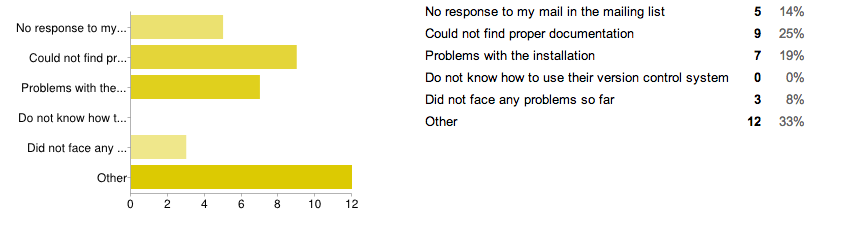
\includegraphics[width=130mm]{chapters/img/problems_faced.png}
\caption{Problems faced by new contributors}
\label{overflow}
\end{figure}

Other major problems which members reported is the lack of sense of community in the open source projects they are trying to contribute. Some complained that they did not get any response or favorable warm response if at all, to their introduction mail in the mailing list. This led to a sense of alienation and fear of contribution in the newbies. 

